\begin{thesischapter}{3} {Análisis de resultados}
    En este capítulo se exponen las funcionalidades que ofrece la aplicación a través de un flujo de uso 
    normal para iniciar una rutina de entrenamiento.  Además, se describirán las estrategias de prueba que se utilizarán para evaluar la efectividad y la 
    usabilidad de la aplicación de juego serio. Se discutirán los métodos de evaluación, como pruebas de usuario 
    y estudios piloto, para recopilar datos cualitativos y cuantitativos sobre la experiencia de los especialistas y pacientes. 
    Además, se considerarán las métricas de rendimiento y los indicadores de progreso para medir el impacto terapéutico de la 
    aplicación.

    \subthesischapter{Comprobación de Requisitos del sistema}

    \subsubthesischapter{Requisitos funcionales}
    A continuación, se muestra el flujo normal, asociado a la ejecución de una rutina
    de juego serio, partiendo del estado en el que el sistema no está iniciado (este flujo de trabajo,
    teóricamente, sería el más utilizado una vez implementado el sistema):

    \begin{figure}[ht]
        \centering
        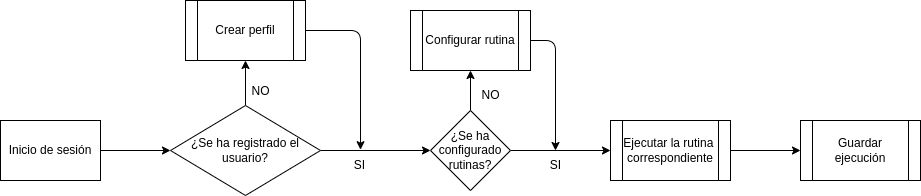
\includegraphics[scale=0.5]{images/diagram-flow.png}
        \caption{}
        \label{fig: diagram-flow}
    \end{figure}
    
    \vspace{10pt}
    Para comenzar, el usuario debe ingresar sus credenciales en la interfaz de Inicio de Sesión, ver figura \ref{fig: ui0} a)
    de no poseer alguna cuenta de usuario registrada en el sistema quedará pasar a la interfaz de registro  
    y registrar un nuevo usuario, ver figura \ref{fig: ui0} b).

    \begin{figure}[ht]
        \centering
        
\includegraphics[scale=0.17]{images/ui/0.jpg}
        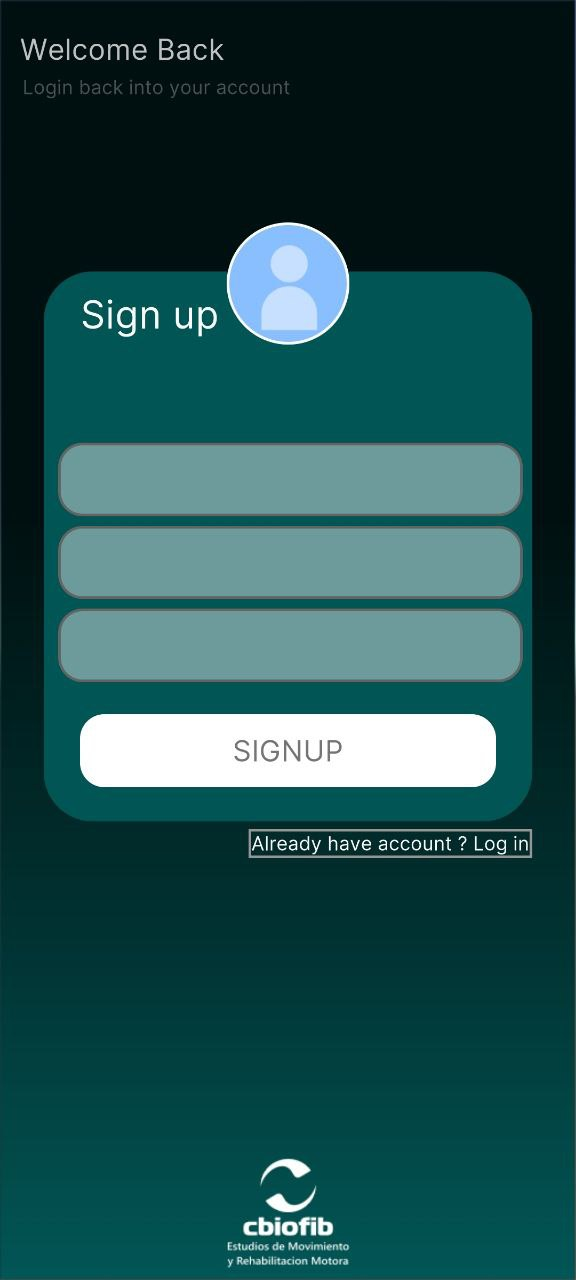
\includegraphics[scale=0.17]{images/ui/1.jpg}
        \caption{a) Vista para el inicio de sesión b) Vista para el registro de usuario}
        \label{fig: ui0}
    \end{figure}

    Después de iniciar sesión se puede se muestra la vista principal donde el usuario puede:
    \begin{itemize}
        \item Configurar e iniciar un entrenamiento.
        \item Iniciar calibración.
        \item Revisar estadísticas.
        \item Revisar y editar datos del perfil. 
    \end{itemize} 

    \begin{figure}[ht]
        \centering
        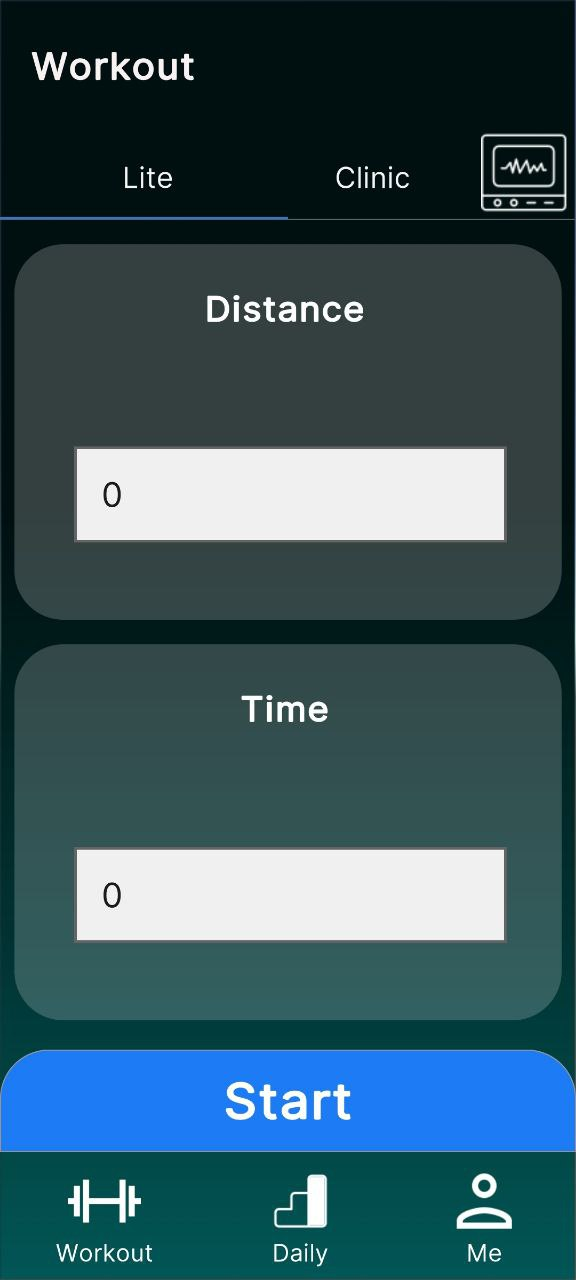
\includegraphics[scale=0.17]{images/ui/2.jpg}
        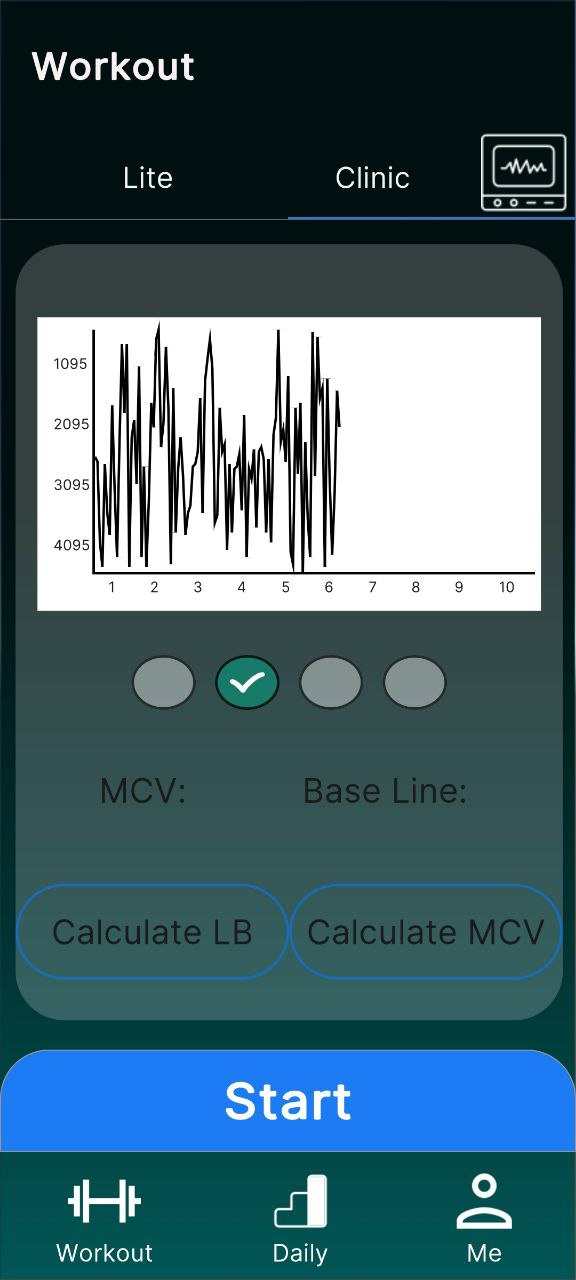
\includegraphics[scale=0.17]{images/ui/4.jpg}
        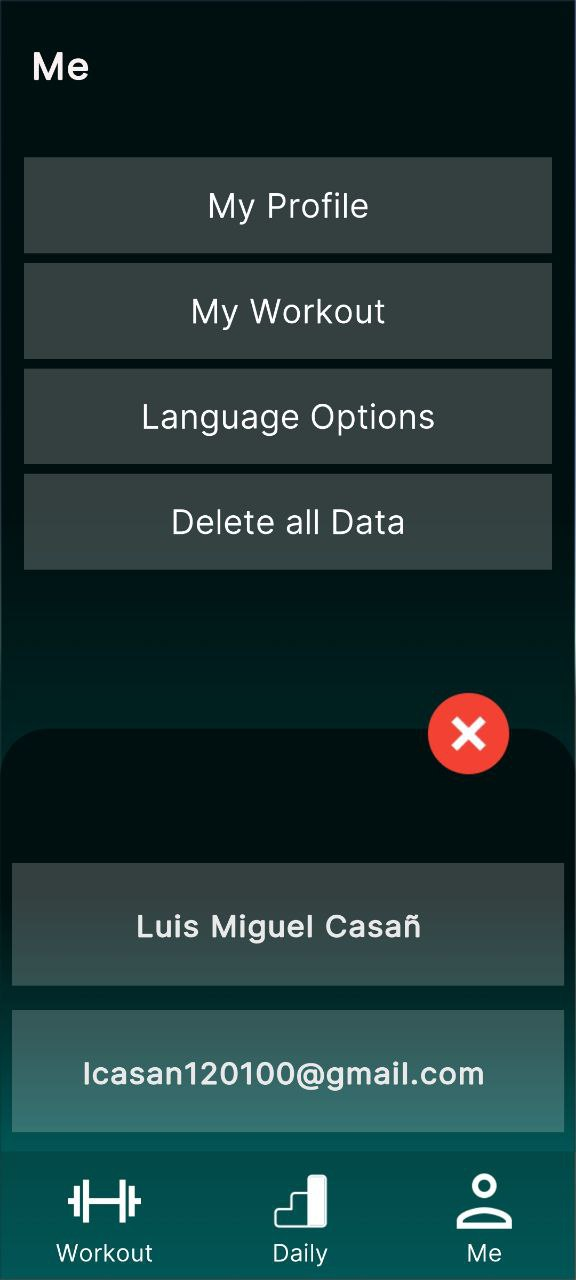
\includegraphics[scale=0.17]{images/ui/3.jpg}
        \caption{Vista principal del usuario}
        \label{fig: ui1}
    \end{figure}


    \vspace{10pt}
    \begin{figure}[ht]
        \centering
        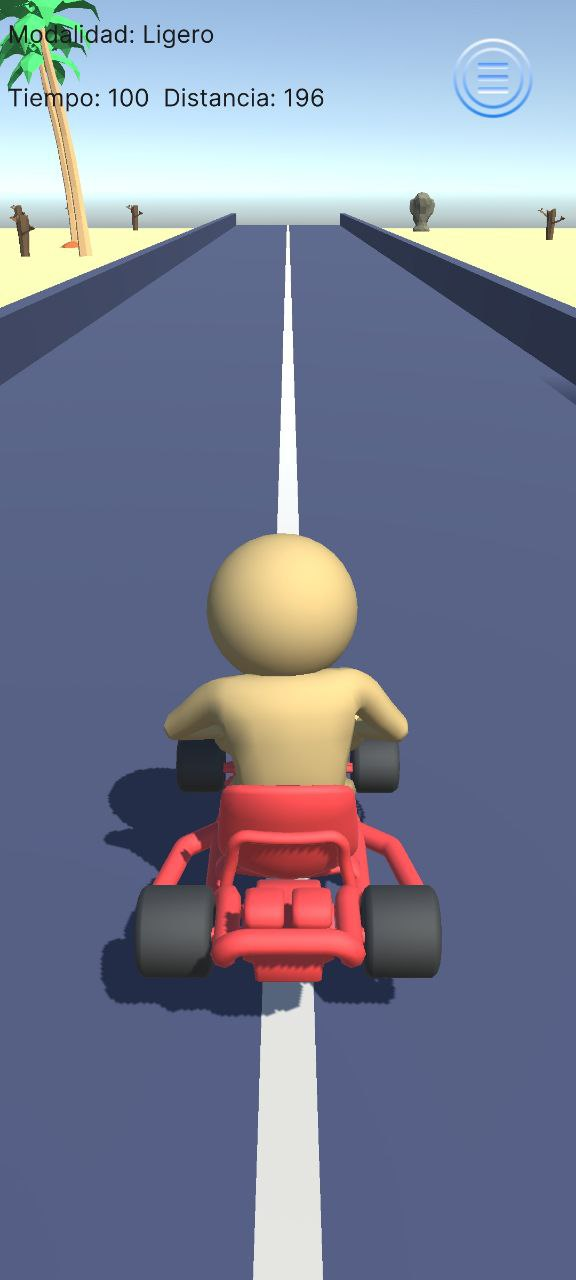
\includegraphics[scale=0.17]{images/ui/7.jpg}
        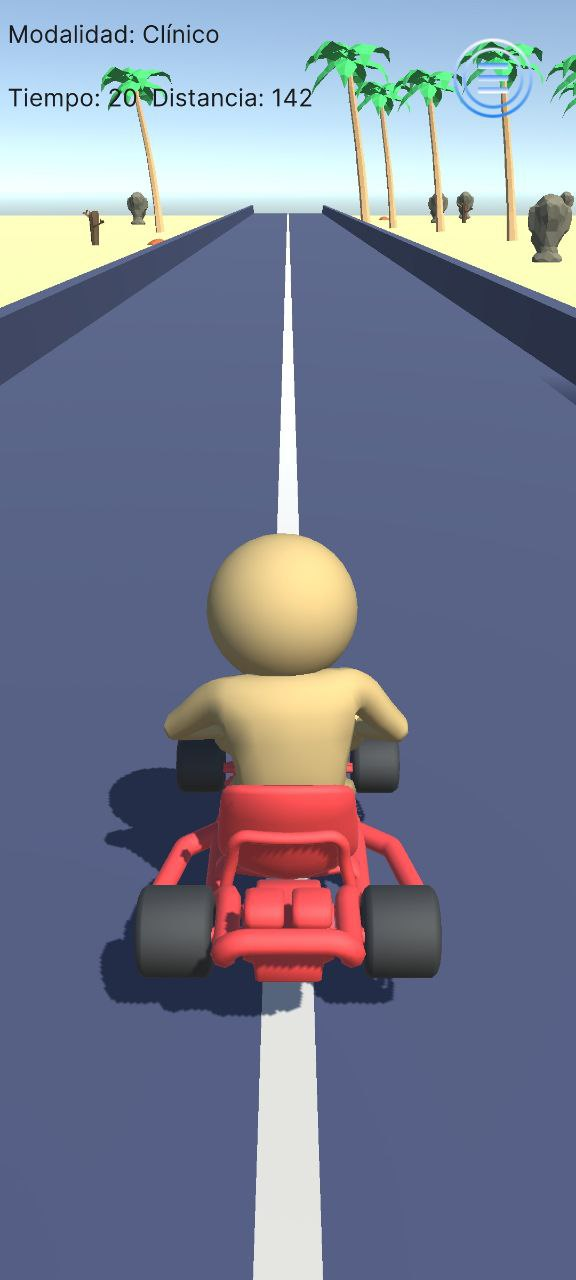
\includegraphics[scale=0.17]{images/ui/6.jpg}
        \caption{a) Escenario ligero b) Escenario clínico}
        \label{fig: diagram-game}
    \end{figure}

    \newpage 
    \subsubthesischapter{Requisitos no funcionales}
    \subthesischapter{Encuesta a especialistas sobre la percepsión del sistema}
    Los 10 encuestados son [Nivel profesional de los encuestados]

    Los resultados de la encuesta a los fisioterapeutas en cuanto a ergonomía, seguridad y concordancia 
    de los ejerciciso con los de la terapia tradicional se presentan agrupados en una escala dicotómica
    en la Tabla \ref{table:test}.
    
\vspace{10pt}
\begin{table}[ht]
    \centering
    \begin{tabular}{ |p{3cm}||p{3cm}|p{3cm}|p{3cm}|  }
        \hline
        \multicolumn{4}{|c|}{Encuesta} \\
        \hline
        &     &  3 &  \\
        \hline
         &     &    &\\
        \hline        
    \end{tabular}
    \label{table:test}

    \caption{Resultados de percepción de fisioterapeutas en cuanto al nivel de}
\end{table}

    \vspace{10pt}
    Las observaciones generales proporcionadas por los fisioterapeutas, permitieron identificar otros 
    potenciales usos en el proceso de rehabilitación


    \vspace{10pt}
    Los hallazgos anteriores van de acuerdo con investigaciones preliminares donde se muestra que con el uso de bicicletas estáticas
    en rehabilitación se puede fortalecer el muñón, mejorar las habilidades de movilidad con la prótesis y mejorar las capacidades 
    aeróbicas del paciente [6], [7], [8].

    \vspace{10pt}
    En gran medida la impresión positiva
    es porque el desarrollo se convierte en un
    reto para el usuario y una ayuda a la
    concentración en una actividad paralela de
    entretenimiento mientras realiza el proceso de
    rehabilitación.
    Si bien se recibieron comentarios negativos
    respecto a la ergonomía en el caso de
    la bicicleta específica utilizada para el
    desarrollo, es decir, con la cual se realizó la
    prueba, especialmente por los inconvenientes
    que traería utilizar dicha bicicleta en una
    persona protetizada en cuanto a estabilidad,
    hubo claridad en los fisioterapeutas que dicha
    situación se soluciona fácilmente adaptando
    el sistema a las bicicletas utilizadas en
    pacientes protetizados, de tipo Recumbent.
    Adicionalmente uno de los encuestados
    expresó sus intentos preliminares a nivel
    personal de implementar una idea parecida
    cuando, mientras realizaba entrenamiento
    físico con una bicicleta estática, practicaba un
    videojuego identificando que lograba mayor
    tiempo de entrenamiento. Una limitación
    que preliminarmente ha sido identificada en
    el sistema es que su uso prolongado, tal como
    sucede en el caso de algunos videojuegos,
    podría contribuir al desarrollo de patologías
    como Tenosinovitis de Quervain, por lo tanto
    es recomendable utilizarlo de acuerdo a las
    recomendaciones del fisioterapeuta.
    Por último, dos fisioterapeutas hicieron
    énfasis en que el sistema solamente se puede
    usar en ciertas etapas de la rehabilitación y
    teniendo en cuenta el nivel de amputación del
    paciente.


\end{thesischapter}